%%%%%%%%%%%%%%%%%%%%%%%%%%%%%%%%%%%%%%%%%
% Programming/Coding Assignment
% LaTeX Template
%
% This template has been downloaded from:
% http://www.latextemplates.com
%
% Original author:
% Ted Pavlic (http://www.tedpavlic.com)
%
% Note:
% The \lipsum[#] commands throughout this template generate dummy text
% to fill the template out. These commands should all be removed when 
% writing assignment content.
%
% This template uses a Perl script as an example snippet of code, most other
% languages are also usable. Configure them in the "CODE INCLUSION 
% CONFIGURATION" section.
%
%%%%%%%%%%%%%%%%%%%%%%%%%%%%%%%%%%%%%%%%%

%----------------------------------------------------------------------------------------
% PACKAGES AND OTHER DOCUMENT CONFIGURATIONS
%----------------------------------------------------------------------------------------

\documentclass{scrartcl}

\usepackage{fancyhdr} % Required for custom headers
\usepackage{extramarks} % Required for headers and footers
\usepackage[usenames,dvipsnames]{color} % Required for custom colors
\usepackage{graphicx} % Required to insert images
\usepackage{listings} % Required for insertion of code
\usepackage{courier} % Required for the courier font
\usepackage{lmodern}
\usepackage{media9}
\usepackage{hyperref}
\usepackage{wrapfig}
\usepackage{listing}
\usepackage{xcolor}

\usepackage[backend=bibtex]{biblatex}
\addbibresource{reference.bib}

\usepackage[T1]{fontenc} % placer ici votre encodage préféré
\usepackage[utf8]{inputenc} % placer ici votre encodage préféré
\usepackage{amsmath}
\usepackage{parskip}
\newcommand{\HRule}{\rule{\linewidth}{0.5mm}}

\graphicspath{ {res/} }

% Margins
\topmargin=-0.45in
\evensidemargin=0in
\oddsidemargin=0in
\textwidth=6.5in
\textheight=9.0in
\headsep=0.25in

\linespread{1.1} % Line spacing

% Set up the header and footer
\pagestyle{fancy}
\rhead{\firstxmark} % Top right header
\lfoot{\lastxmark} % Bottom left footer
\cfoot{} % Bottom center footer
\rfoot{Page\ \thepage} 
\renewcommand\headrulewidth{0.4pt} % Size of the header rule
\renewcommand\footrulewidth{0.4pt} % Size of the footer rule

\setlength\parindent{0pt} % Removes all indentation from paragraphs


%----------------------------------------------------------------------------------------
% DOCUMENT STRUCTURE COMMANDS
% Skip this unless you know what you're doing
%----------------------------------------------------------------------------------------

% Header and footer for when a page split occurs within a problem environment
\newcommand{\enterProblemHeader}[1]{
\nobreak\extramarks{#1}{#1 continued on next page\ldots}\nobreak
\nobreak\extramarks{#1 (continued)}{#1 continued on next page\ldots}\nobreak
}

% Header and footer for when a page split occurs between problem environments
\newcommand{\exitProblemHeader}[1]{
\nobreak\extramarks{#1 (continued)}{#1 continued on next page\ldots}\nobreak
\nobreak\extramarks{#1}{}\nobreak
}

\lstdefinestyle{sharpc}{language=[Sharp]C, frame=lr, rulecolor=\color{blue!80!black}}
\begin{document}


\lstset{style=sharpc}
%----------------------------------------------------------------------------------------
% TITLE PAGE
%----------------------------------------------------------------------------------------

\begin{titlepage}
\begin{center}

% Upper part of the page. The '~' is needed because \\
% only works if a paragraph has started.

\textsc{ Kungliga Tekniska Högskolan \\ School of Computer Science and Communication}\\[1.5cm]

\begin{figure}[ht]
\begin{center}

\includegraphics[width=0.65\textwidth]{KTH}
\end{center}
\end{figure}

\textsc{\Large DH2323}\\[0.5cm]

% Title
\HRule \\[0.4cm]
 { \huge \bfseries A Nice Title \\[0.4cm] }
{\large \bfseries  Project Documentation\\[0.4cm] }

\HRule \\[1.5cm]

% Author and supervisor
\begin{minipage}{0.65\textwidth}
\begin{flushleft} \large
Michael \textsc{Hotan} \\
Alexandre \textsc{St-Onge}\\
\end{flushleft}
\end{minipage}

\vfill

% Bottom of the page
{\large \today}

\end{center}
\end{titlepage}

%----------------------------------------------------------------------------------------
% Introduction
%----------------------------------------------------------------------------------------

\section{Introduction}

	For this project, we designed and implemented a Unity application to simulate bike traffic in a park scene. In phase 1 
	of the project we first created a park scene containing a road, park bench, trees and light sources. In phase 2 we started 
	working on the bike traffic. Finally, in phase 3 we worked on shader to apply to our cyclist model.
	
\section{Documentation}

	\subsection{Rendering a scene in Unity}
		The first step in this project was to create a realistic park scene to use as a background for our application. The simplest 
		way to do this was to use the built-in terrain feature of Unity. With the terrain object we were able to easily obtain a grassy 
		plain with trees and hill. Next we used Jacek Jankowski's street kit\parencite{Street:Jankowski} to setup a road for our future 
		bike traffic. From there, since we knew we wanted to work with some shader for our bike model, we added some street lights that 
		we got from the asset store\parencite{StreetLight:BiSkiT} and some park bench\parencite{Parkchair:Universal}. Appropriate material 
		for the sky were used with Unity's skybox to obtain a nice sky for the scene. For the daylight scenario, a single directionnal light is 
		used for the sun, while the nightime scenario uses one spotlight attached to each of the four street lights.
		
		\begin{figure}[h]
			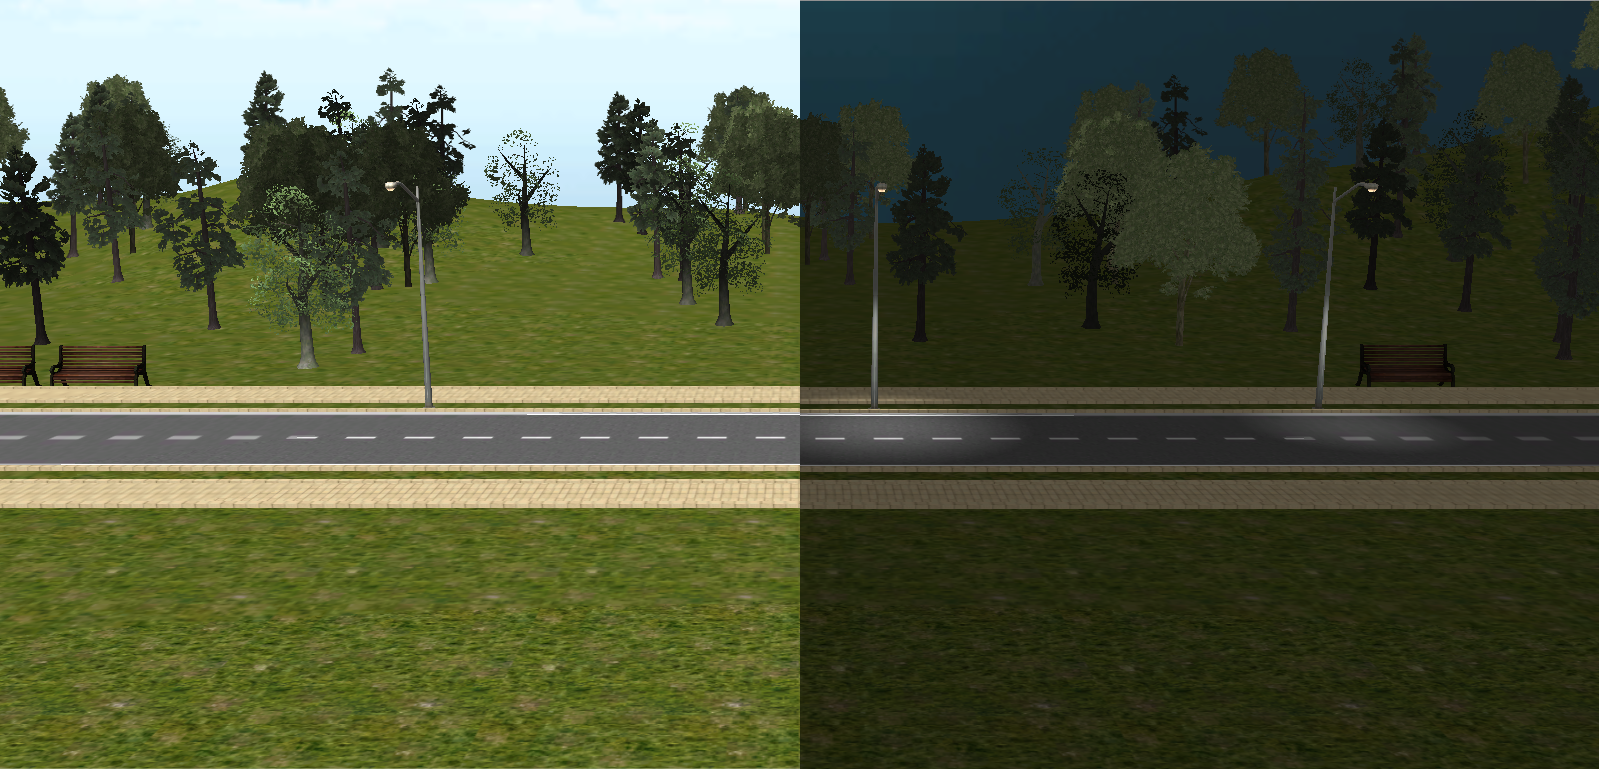
\includegraphics[width=\textwidth]{parkDayNight}
			\caption{Park scene in Unity}
			\label{fig:park_scene}
		\end{figure}
		
	\subsection{Rendering the cyclist}
		Next step in our project was to find a 3d model for the bike and the cyclist. We used a 3d model from \url{www.blendswap.com} \parencite{Bicycle:Blender}, as 
		seen in figure~\ref{fig:bike_model}. The model already had a basic animation so it was perfect for our need. Since it 
		was a blender file, using it in Unity was not very simple. First, the animation needed to be adapted for our need. I had to change the 
		animation slightly to make it more "loopable" in Unity. Also, the initial animation had the model moving forward, causing it to "teleport" 
		back to its initial position at every loop, I then changed it so the animation now plays in-place. Having in-place animation is needed 
		since we wanted to use Unity to move the bike ourselves. Once everything looked great in blender, the model was loaded into our Unity 
		project. The bike was then scaled and rotated accordingly and was saved into what Unity call a "prefab". Having the model as a prefab allow 
		us to easily instantiate the model during runtime. 
		\begin{figure}[h]
			\includemedia[
				label=bike2.u3d,
				3Daac=60.000000, 
				3Droll=90.000000 , 
				3Dc2c=85.835000 60.632999 45.966000, 
				3Droo=42.717735, 3Dcoo=1.834687 3.523406 -1.965973
				]{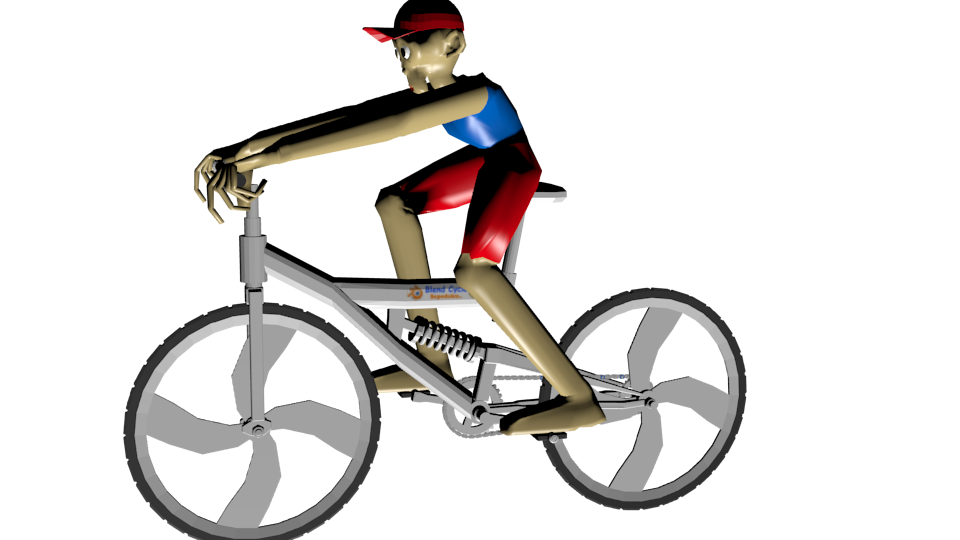
\includegraphics[width=0.8\textwidth]{BikeModel}}{res/bike2.u3d}
			\caption{Bike 3d model found on \url{blendswap.com}}
			\label{fig:bike_model}
		\end{figure}
		
	\subsection{Generating Traffic}
		The final step was to generate traffic. There is multiple way to do this. The first method we try was simply to add a rigidbody onto the bike and 
		add a constant force in the direction we want with a script. Since the animation is automatically playing and looping, this is a simple and easy way 
		to have a bike rolling from one point to the other in a straight line. As the density of bike goes up, the chance of collision is much higher too and 
		since we have not implemented any path-finding the simulation quickly becomes a mess. Luckily, Unity provides us with a built-in pathfinding solution 
		with NavMeshAgent. First I had to define the navigable area in the scene with a NavMesh. We can do this in the navigation window in Unity by disabling 
		navigation for the terrain and enabling it for our set of road. Next, we need a target and a spawn point for our bike. We can create these with simple 
		empty GameObject placed at the appropriate position. We can then add a NavMeshAgent on our bike prefab. We now have to setup the agent with a script.
		This is done in NavBike.cs in the Update() method with a simple line of code: 
		
		\begin{lstlisting}
		    agent.SetDestination(target.position);
		\end{lstlisting}
		
		Once the destination is set, the agent will move the object toward the target while avoiding any obstacles (i.e.: other bikes)  in the way. Now that we 
		have a simple way of moving bike from one side to the other we can work on making the traffic nicer. This is done in the GenerateBike.cs script. I modeled 
		the traffic according to a simple equation where the flow is equal \textbf{u*k} where \textbf{k} is the number of vehicles per unit of distance and \textbf{u} 
		is the average speed of the vehicles. To be able to observe how these two variables affect the flow, I use two sliders: one for the density and one for the speed. 
		If we want more bikes per distance we need to spawn more bikes, this is done by sliding the density slider to the right. The slider affect the intervals between each 
		spawn. The Random.Range function is used to make the spawn intervals look more natural. The next slider affect the bike's speed. Before being instantiated, each bike 
		is assign a speed randomly chosen in an interval around the slider's value. This allow us to choose the average speed with the slider, while still having faster and slower 
		bike. The ComputeFlow() method is there to quantify the traffic flow so we can show it on screen. The flow is calculated using the equation presented earlier.
		
		\begin{figure}[h]
			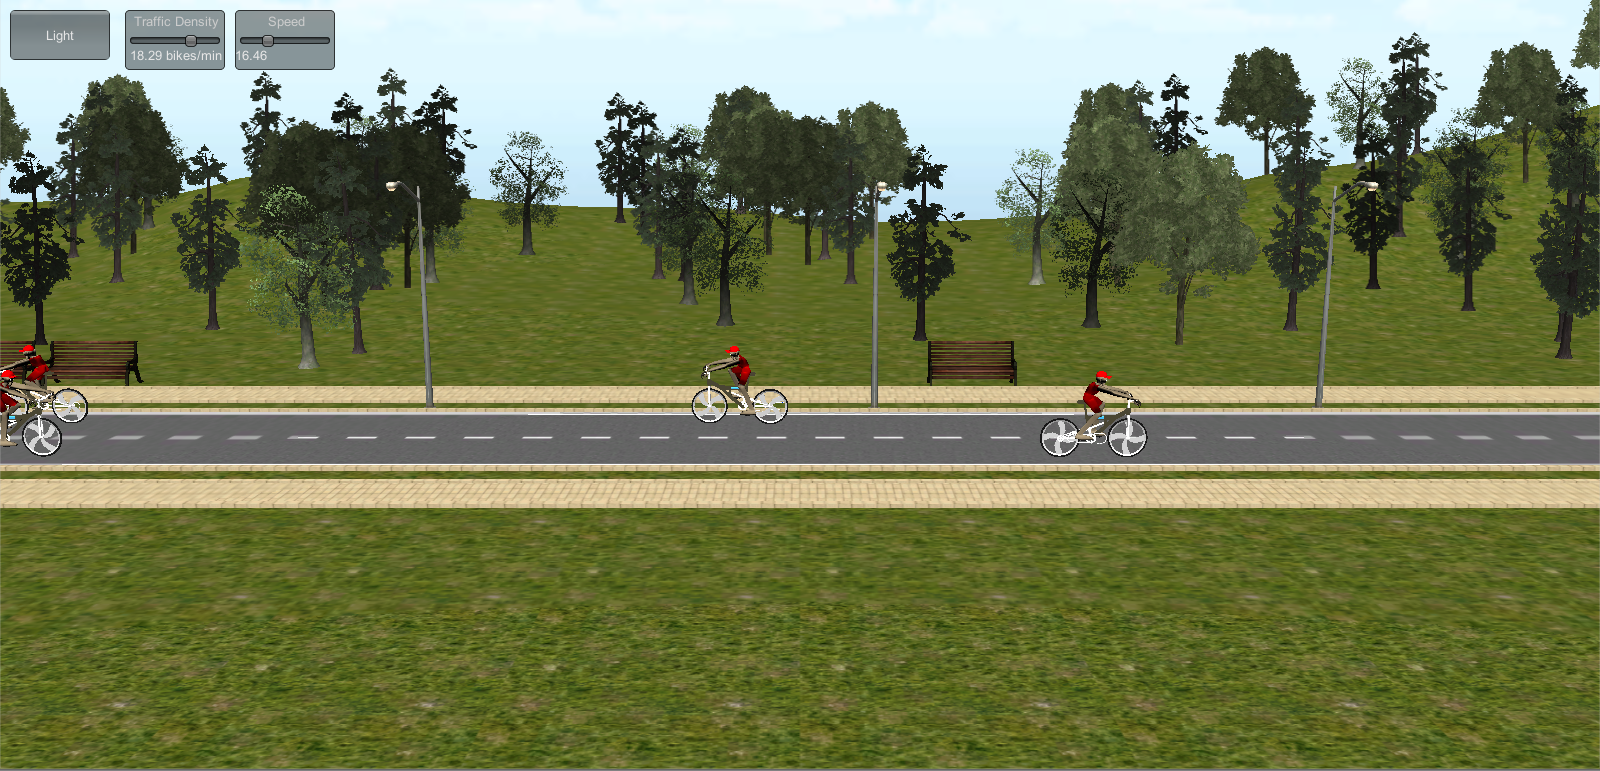
\includegraphics[width=\textwidth]{AppWithGUI}
			\caption{Screenshot of the application running with the GUI in the top left corner}
			\label{fig:app_gui}
		\end{figure}
		
	\subsection{Conclusion}
		For this project I had the responsibility of generating bike traffic at runtime in a realistic manner. While my partner is working on finding realisic way of rendering 
		the scene with shader, I was in charge of finding a realistic traffic flow. While there is a lot of research done on the subject of traffic flow for computer generated 
		scene, a lot of them were too much complex for my level of understanding and I found that they didn't really apply to our scenario. Indeed, bike traffic is very 
		different from car traffic. Car traffic is organized, dense and follow a numbers of well defined rules. On the other hand, bike traffic is a lot more sparse and organic. 
		I actually spend some times in parks observing bike traffic for this project and observe a low traffic flow at around 8 or 10 bikes per minutes. The speed variation 
		between bikes is also considerable, which is why I used a random number generator to assign speed over an interval instead of using the same speed for everyone. 
		Working on this project allowed me to learn about how to create scene with a framework like Unity. It can be difficult to put all these 3d models together, you have 
		to think about scale, positions and rotation, and if you want to generate object by script you need to understand these concept even more. By choosing to use the 
		navigation framework provided by Unity, my goal was to make sometime reusable and I'm confident that my work could be easily in any scene where you would want 
		to add bike traffic between two points.
		
\section{Perception Studies}


\printbibliography

\end{document}

